\section*{2.1 Cart-Pole Swing-Up with Limited Actuation}

\subsection*{2.1(a)}
We want the constraint $s_{k+1}=f_{\text{d}}(s_k,u_k)$ to have the form $s_{k+1}=A_k s_k+B_k u_k+c_k$ to derive the convex approximation of the OCP at iteration \(i\), around \((s_k^{(i)},u_k^{(i)})\).

The linearization of $f_{\text{d}}(s_k,u_k)$ becomes:
$$
f_{\text{d}}(s^{(i)}_k,u^{(i)}_k) =
f_(s^{(i)}_k,u^{(i)}_k) + \frac{\partial f_d}{\partial s}(s_k^{(i)},u_k^{(i)}) (s_k - s^{(i)}) +  \frac{\partial f_d}{\partial u}(s_k^{(i)},u_k^{(i)})(u_k - u^{(i)})
$$
After expanding terms, we come up with
\[
    A_k=\frac{\partial f_d}{\partial s}(s_k^{(i)},u_k^{(i)}),\qquad
    B_k=\frac{\partial f_d}{\partial u}(s_k^{(i)},u_k^{(i)}),
\]
\[
    c_k=f_d(s_k^{(i)},u_k^{(i)})-A_k s_k^{(i)}-B_k u_k^{(i)}.
\]
The convex subproblem is
\[
\begin{aligned}
\min_{s,u}\quad
&\sum_{k=0}^{N-1}\left((s_k-s_{\rm goal})^TQ(s_k-s_{\rm goal})+u_k^TRu_k\right)
 +(s_N-s_{\rm goal})^TP(s_N-s_{\rm goal})\\
\text{s.t.}\quad
&s_0=\bar s_0,\\
&s_{k+1}=A_k s_k+B_k u_k+c_k,\\
&-u_{\max}\le u_k\le u_{\max},\\
&\|s_k-s_k^{(i)}\|_\infty\le \rho,\qquad
  \|u_k-u_k^{(i)}\|_\infty\le \rho.
\end{aligned}
\]

\subsection*{2.1(b)}
\begin{lstlisting}
A, B = jax.jacobian(f, argnums=(0, 1))(s, u)
c = f(s, u) - A @ s - B @ u
\end{lstlisting}

\subsection*{2.1(d)}
First use SCP to compute a feasible swing-up trajectory. Once the pendulum is near
\((0,\pi,0,0)\), switch to a local LQR controller designed around \((0,\pi,0,0)\) for stabilization.

\begin{figure}[H]
\centering
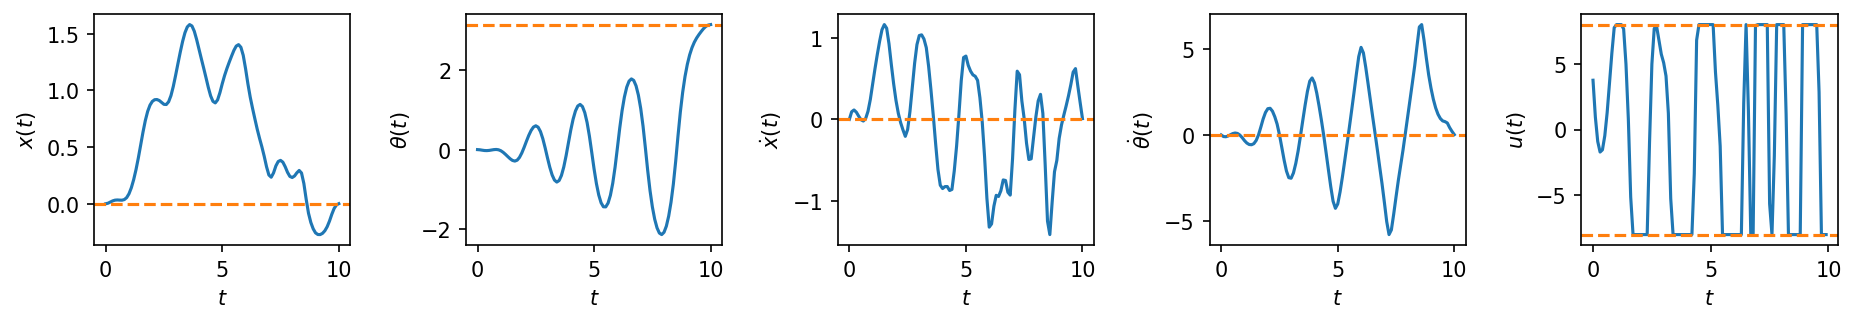
\includegraphics[width=\textwidth]{figures/cartpole_swingup_constrained.png}
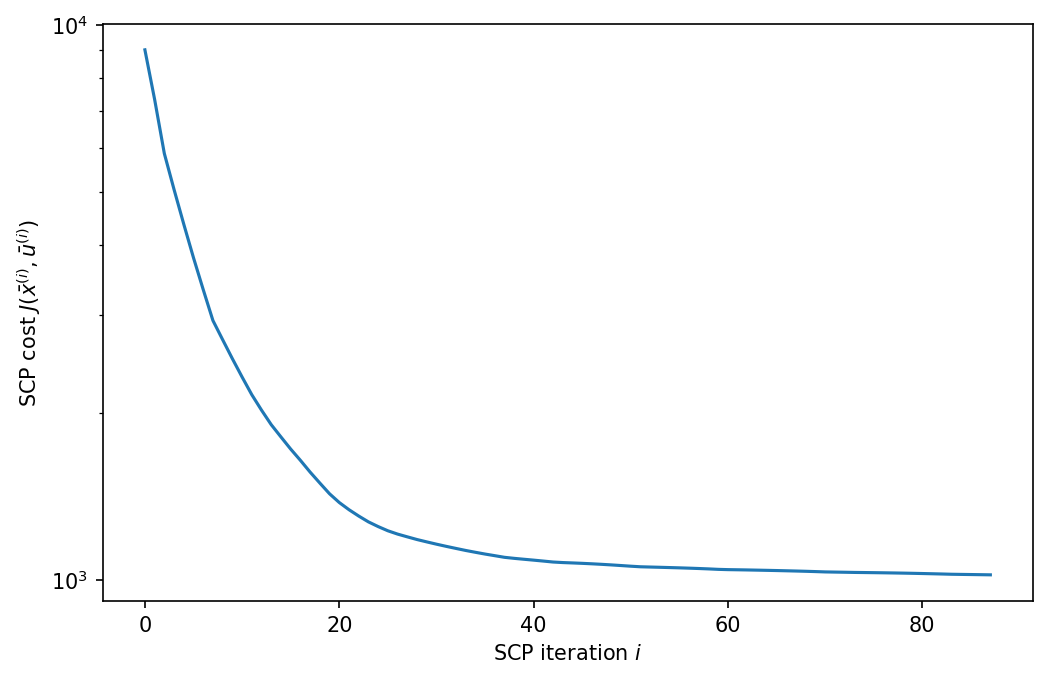
\includegraphics[width=0.65\textwidth]{figures/cartpole_swingup_constrained_cost.png}
\caption{SCP swing-up trajectory with bounded input and trust-region updates.}
\end{figure}

\subsection*{Code}
Code in Appendix: \hyperref[cartpole_swingup_constrained]{\texttt{cartpole\_swingup\_constrained.py}}.
